\chapter{Fundamentação teórica}

\label{conceitos-fundamentais}

%\input{Content/trabalhos.tex}
Neste capítulo é apresentada a fundamentação teórica utilizada para o desenvolvimento do trabalho. Ele apresenta os conceitos básicos de inteligência artificial e um estudo aprofundado sobre agentes e percepções. Além disso, este capítulo apresenta definições que serão utilizadas na formalização do modelo no Capítulo \ref{chapter:model}.

\section{Inteligência artificial}

A Inteligência Artificial é um campo de estudo que se difere, pois enquanto outros campos do conhecimento se limitam a buscar entender \textit{como} o pensamento humano funciona, a IA se propõe a construir entidades pensantes \cite{russel2013artificial}. Apesar de ser uma área de pesquisa que surgiu na década de 50 \cite{moor2006dartmouth}, não existe uma única definição de Inteligência Artificial nem consenso dentro da comunidade acadêmica.

Uma visão prática do que é IA é sua abordagem como a automatização de diversas tarefas humanas: ``atividades que associamos ao pensamento humano, atividades como a tomada de decisões, a resolução de problemas, o aprendizado'' \cite{bellman1978introduction}. Essa definição é derivada da pergunta ``computadores podem pensar?''. Existem diversos exemplos de atividades do pensamento humano que os computadores são capazes de executar, como tratamento de incerteza, consciência e humor. Apesar disso, para Bellman, ``o espírito humano se mantém muito acima de qualquer coisa que possa ser automatizada''. Essa é uma visão de que o objetivo da IA é replicar o pensamento humano.

Um outro ponto de vista coloca a IA como ferramenta de investigação da mente humana, ou seja, como ``o estudo das faculdades mentais através do uso de modelos computacionais'' \cite{charniak1985introduction}. Para essa definição estar correta é necessário que exista uma equivalência entre o processo mental humano e o processamento de um computador. Por conta disso, Charniak define o dogma central da Inteligência Artificial: ``O que o cérebro faz pode ser pensado em algum nível como um tipo de computação''. Caso o dogma se mostre verdadeiro, o uso de modelos computacionais para o estudo das faculdades mentais é valido. ``Faculdades mentas'', dentro dessa definição, são os mecanismos internos que recebem imagens e palavras (através da visão e da linguagem) e os converte em saídas na forma de ações robóticas e fala. Esse processamento interno inclui dedução, planejamento, aprendizado e outras técnicas.

As definições de IA podem ser divididas entre aquelas que defendem que os computadores devem pensar como humanos, e aquelas que defendem que os computadores devem agir como humanos \cite{russel2013artificial}. As duas definições apresentadas anteriormente estão no primeiro grupo. As definições que levam em conta que os computadores devem agir como humanos em geral possuem um aspecto mais prático. Por exemplo, a definição dos autores Rich e Knight diz que inteligência artificial é ``o estudo de como os computadores podem desempenhar tarefas que hoje são melhor desempenhadas pelas pessoas'' \cite{rich1991artificial}. Com isso podemos notar que esse lado mais prático da IA não precisa se preocupar tanto com as questões filosóficas por trás do pensamento humano, pois foca em resolver problemas reais através dos métodos existentes. 

Neste trabalho, utilizaremos uma definição nessa mesma linha de pensamento de que o computador deve agir como um ser humano, nesse caso específico, de maneira lógica: ``inteligência computacional é o estudo do desenvolvimento de agentes inteligentes'' \cite{poole1998computational}. Essa definição foi escolhida pois o HAIL se trata de um modelo desenvolvido para agentes inteligentes. A Seção \ref{section:agent} se dedica a definir o que é um agente.

Independente da definição utilizada, podemos afirmar que a IA é um campo vasto que intriga muitos pesquisadores. Esse campo possui diversas técnicas, que são utilizadas para resolver todo o tipo de problemas. Kurzweil apresenta a seguinte visão sobre a pesquisa de Inteligência Artificial:

\begin{displayquote}
    É nosso destino como pesquisadores de Inteligência Artificial nunca alcançar a cenoura pendurada à nossa frente. A inteligência artificial é inerentemente definida como a busca de problemas difíceis da ciência dos computadores que ainda não foram resolvidos \cite{kurzweil2000age}.
\end{displayquote}



\section{Agente inteligente}

\label{section:agent}

Um agente inteligente é uma entidade autônoma, capaz de tomar as próprias decisões para atingir seus objetivos \cite{wooldridge1999intelligent}. Apesar da definição intuitiva ser simples, assim como no termo inteligência artificial não existe um consenso da comunidade sobre o que é um agente. Definições mais simples categorizam agente como algo que age, e agente inteligente como aquele que age buscando o melhor resultado possível \cite{russel2013artificial}, enquanto definições mais fechadas buscam contextualizar a entidade em um ambiente:

\begin{displayquote}
    Um agente inteligente é um sistema que age de maneira inteligente: o que faz é apropriado para as circunstâncias e seus objetivos, é flexível para mudar ambientes e mudar objetivos, aprende com a experiência e faz escolhas apropriadas, dadas as limitações perceptivas e a computação finita \cite{poole1998computational}.
\end{displayquote}

Tais definições são bastante amplas, e enquadram diversos tipos de programas computacionais. Apesar disso, agentes possuem características específicas, principalmente provenientes da capacidade de interagir uns com os outros. As capacidades e características dos agentes inteligentes podem ser divididas em cinco tópicos \cite{lugerBook6th}: 

\begin{enumerate}
    \item \textbf{Agentes são autônomos ou semi-autônomos:} Os agentes são independentes, ou seja, cada agente é capaz de trabalhar em uma tarefa sem saber no que outros agentes estão trabalhando, ou sem saber como eles resolvem determinada tarefa. Além disso, eles podem tanto fazer algo efetivamente (agir) ou reportar seus resultados para outros agentes (se comunicar).
    \item \textbf{Agentes possuem escopo localizado:} Cada agente é sensível ao ambiente, e normalmente não possui conhecimento sobre aquilo que todos os outros agentes estão realizando. Portanto o conhecimento de um agente é limitado às tarefas que ele deve realizar, sem conhecimento amplo sobre seus limites.
    \item \textbf{Agentes são interativos:} Normalmente, agentes se agrupam em forma de sociedade, com o objetivo de colaborar para resolver um problema. E assim como na sociedade humana, o conhecimento, a responsabilidade, habilidades e outros recursos estão distribuídos entre os indivíduos.
    \item \textbf{As sociedades dos agentes são estruturadas:} Na maioria das abordagens de solução de problema orientada a agentes, cada agente, mesmo possuindo seu próprio conjunto de habilidades e objetivos, se coordena com outros agentes para a resolução geral de problemas. Portanto, a solução final não é apenas coletiva, mas também cooperativa.
    \item \textbf{O fenômeno da inteligência nesses ambientes é emergente:} A capacidade final da resolução de um problema por uma sociedade de agentes é maior do que a soma das capacidades individuais de trabalho. A inteligência é vista como um fenômeno residente e emergente de uma sociedade e não apenas uma propriedade de um agente individual.
    
\end{enumerate}

A noção de agente inteligente ainda pode ser caracterizada como forte ou fraca \cite{wooldridge1995intelligent}. A noção fraca de agente é utilizada para denominar hardware ou software que possui algumas características específicas, sendo elas autonomia, habilidade social, reatividade e pró-atividade. Já a noção forte de agente se refere a um sistema que, além das características citadas anteriormente, ou foi concebida ou foi implementada utilizando conceitos que normalmente se aplicam a humanos. O modelo explorado neste trabalho segue a noção forte de agente, pois se baseia em conceitos da psicologia e da filosofia para resolver um problema prático de agentes.

Com base na leitura das definições apresentadas anteriormente, para este trabalho vamos definir agente formalmente conforme apresentado na Definição \ref{def:agent}, de maneira que facilite a manipulação e formalização do modelo proposto.

\theoremstyle{definition}
\begin{definition}
    \label{def:agent}
    Um agente é uma tripla $Ag = \langle K, P, \gamma \rangle$, onde:
    \begin{itemize}
        \item $K$ é uma base de conhecimentos, tal que $K = K_i \cup K_p$, onde $K_i$ é o conjunto de conhecimentos inicias do agente e $K_p$ os conhecimentos adquiridos através das percepções. $K_i$ é iniciado com valores arbitrários de acordo com a necessidade do agente e $K_p$ é iniciado vazio. Uma base de conhecimentos é uma estrutura que representa fatos a respeito do mundo e apresenta formas de raciocinar a respeito desses fatos para deduzir novos conhecimentos \cite{hayes1983building};
        \item $P$ é o conjunto de planos do agente, sendo um plano definido como $plano = (\Psi, A, \Omega)$, onde $\Psi$ é o conjunto união formado pelas pré-condições das ações que compõem o plano, $A$ o conjunto de ações que compõe o plano e $\Omega$ o conjunto união formado pelas pós-condições das ações que compõem o plano. Por sua vez, uma ação é definida como $acao = (\psi, n, \omega)$, sendo $\psi$ um conjunto de pré-condições, $n$ um nome para a ação e $\omega$ um conjunto de pós-condições; e
        \item $\gamma$ é a função de percepção, definida como $ \gamma(p, K) \rightarrow P_i $, onde $p$ é o conjunto de percepções recebidas, $K$ a base de conhecimentos de $Ag$ e $P_i$ o retorno da função, que é um subconjunto próprio do conjunto $P$ de planos do agente.
    \end{itemize}{}
\end{definition}{}

A partir dessa definição, podemos construir o conceito de contexto, que será amplamente utilizado na formalização do modelo de revisão de percepções. O contexto de um agente é o conjunto de todos os símbolos compreendidos pelo agente:

\begin{definition}
    O contexto $c$ de um agente $Ag$ é o domínio de sua função $\gamma$.
    \label{definition::context}
\end{definition}{}



\iffalse
\section{Agente}

Essa seção é um esqueleto de uma definição de agente que pode ser útil para explicar o modelo proposto. O foco é a relação da função $\Lambda$ com o resto do modelo, portanto K, A e P precisam ser melhorados.

Para esse artigo vamos definir agente como a quádrupla $Ag = (K, A, P, \Lambda)$, onde:

\begin{itemize}
    \item K é o conjunto de conhecimentos que o agente possui, podendo ter adquirido ou já ter começado com eles. Essas conhecimentos podem se referir a coisas que o agente conhece do mundo, coisas que o agente quer mudar no mundo ou coisas abstratas.
    \item A é o conjunto de atuadores do agente, ou seja, coisas que o agente pode usar para causar mudança no mundo (e, portanto, nos conhecimentos K).
    \item P é o conjunto de percebedores do agente, que adquirem novas informações a respeito do ambiente, causando mudança em K.
    \item $\Lambda$ é a função de percepção, que opera sobre a entrada de P, baseado nas informações contidas em K e retorna um subconjunto de A.
    \[ \Lambda: P \times K \rightarrow 2^A\]
\end{itemize}

Eu não sei se o jeito que eu escrevi está certo, mas usando essa ideia o que foi chamado de Contexto no resto do artigo pode ser facilmente definido como a imagem da função $\Lambda$.

\fi

\section{Percepção}

Existem diversas definições para o termo ``percepção''. Podemos entender percepção como um conjunto de sensações que, através da maneira subjetiva que um dado agente o interpreta, representa determinadas entidades do ambiente \cite{gibson1950perception}. Ou seja, a percepção não é simplesmente a representação direta das entidades reais que existem no mundo, mas um processo complexo que varia para cada indivíduo.

Percepções podem ser divididas nos níveis baixo e alto \cite{chalmers1992high}. A percepção de baixo nível ocorre através de meios físicos, os órgãos ópticos para os humanos ou os sensores para os agentes. 
A percepção de alto nível trabalha com uma visão mais geral da informação, extraindo conceitos dos dados brutos, podendo envolver diversas faculdades como o reconhecimento de objetos e o relacionamento de entidades. Nos trabalhos de Inteligência Artificial, em geral, estamos interessados na percepção de alto nível, pois a percepção de baixo nível está mais relacionada a robótica (no caso de agentes que possuem hardware próprio) ou a simulação (no caso de agentes que possuem apenas software).

Ainda segundo Chalmers et. al. uma das principais características da percepção de alto nível é a extrema flexibilidade. Um mesmo objeto do ambiente pode ser percebido de diversas maneiras, de acordo com as características do observador. Para os autores, algumas das fontes da flexibilidade das percepções são a capacidade de serem influenciadas pelas crenças, objetivos e contexto externo. Além disso, percepções de um mesmo objeto podem ser radicalmente alteradas conforme o necessário.

Para o modelo que iremos propor, baseado na Definição \ref{def:agent}, o conceito de percepção pode ser simplesmente definido como a entrada $p$ da função de percepção $\gamma$ de um agente. Vale destacar a diferença entre percepção e contexto, pois o contexto é constituído pelas percepções que fazem parte do domínio da função $\gamma$, ou seja, uma percepção é toda informação produzida pelo ambiente que o agente recebe, e contexto é o subconjunto das percepções que o agente reconhece.

Em ambientes dinâmicos há possivelmente centenas de percepções por segundo \cite{hayes1992guardian}. Mas percepções não necessariamente precisam incluir representações corretas da realidade e podem variar de agente para agente \cite{janssen2005agent}. Percepções incorretas podem ocorrer por conta de limitações da capacidade do agente de perceber determinados objetos ou por conta de obstrução física dos sensores, por exemplo \cite{chrisman1991intelligent}.

\subsection{Refinamento}

Como o volume de percepções de um agente pode ser muito grande, e as percepções custam tempo para serem processadas, o número de percepções que chegam ao ciclo de raciocínio do agente pode ser reduzido para diminuir seu custo computacional. Neste trabalho, esse processo será chamado de refinamento, definido da seguinte maneira:

\begin{definition}
    \label{def:refinamento}
    Refinamento de percepções é uma função $\theta$ tal que, dado o conjunto de entradas de percepções $p$, reduz tais percepções para um subconjunto próprio $\rho$.
\end{definition}

Existem diversas maneiras de realizar refinamento. Uma das mais clássicas é o uso de filtros de percepções, que limitam que percepções serão processados pelo agente baseado em diversos critérios, como posição, distância e a velocidade do objeto percebido \cite{bordeux2001}. Outra maneira de restringir as percepções é a percepção ativa. Um observador pode ser categorizado como ativo se ele ativamente pode executar uma ação que altere as configurações geométricas de seus sensores, com objetivo de melhorar a qualidade de sua observação \cite{Aloimonos1988}. O processo realizado pela percepção ativa pode ser definido através da tupla: por quê, o que, quando, onde e como perceber  \cite{Bajcsy2018}. Desta maneira, o agente pode perceber apenas quando é necessário (por quê), escolhendo o que perceber (o que) e otimizar fisicamente a percepção (quando, onde e como).

\subsection{Anomalias}

Anomalias são as percepções consideradas inválidas, geradas por alguma falha no processo de percepção. O conjunto de anomalias de um agente é o conjunto de todas as percepções possíveis que não fazem parte de seu contexto. A seguinte definição será utilizada:

\begin{definition}
    Uma percepção $p$ de um agente $Ag$ com contexto $c$, é uma anomalia caso $p \notin c$ de $Ag$.
\end{definition}

Anomalias podem ser divididas em dois tipos: alucinações e ilusões. Nas seções seguintes, será descrito o que as alucinações e ilusões são para os estudos clássicos do problema da percepção \cite{Russell1912-RUSTPO-49} \cite{Price1933-PRIP-20} e como elas podem ser representadas dentro do processo de percepção de agentes inteligentes. A base desse estudo foi o artigo ``The Problem of Perception'' \cite{perception-problem}.

\subsubsection{Ilusão}

Uma ilusão, na definição clássica onde o objeto de estudo são os seres humanos, é qualquer situação perceptiva na qual um objeto físico é realmente percebido, mas ele aparenta ser outra coisa que ele não é \cite{Smith2002-SMITPO-17}. O Exemplo \ref{example::ilusao1} ilustra o que é uma ilusão.

%Essa definição será usada como base para criar nossa definição computacional para ilusão. Entretanto, é importante notar que essa é uma definição diferente de outras encontradas na literatura, como a usada por Lhelani et. al. \cite{Khemlani2017}, onde uma ilusão é uma falácia advinda de uma interpretação humana errada sobre um problema lógico resolvido pelo computador.

\begin{example}{}
Suponha um robô que possui a tarefa de empacotar diferentes itens do depósito de uma loja. Os itens passam por uma esteira, e o agente usa dois sensores para perceber o que os itens são. O primeiro sensor é uma câmera ligada ao topo do corpo do robô, usado para definir a forma do item. O segundo sensor é um detector de textura na lateral das esteiras. Assim, as informações advindas dos sensores formam predicados da forma \texttt{forma(textura)}, que descreve um item. Os itens podem ter a forma de um círculo, um quadrado ou um triângulo, e sua textura pode ser lisa ou listrada.
O agente possui duas cores de papéis para empacotar, vermelho e azul. O papel vermelho é usado para quadrados (de ambas as texturas) e círculos lisos. O papel azul é usado para círculos listrados e triângulos lisos. A loja não vende triângulos listrados, então não há nenhum item desse tipo no depósito. Podemos descrever esse comportamento com as seguintes regras:

\begin{center}
    \texttt{papel(vermelho) :- quadrado(\_) OR circulo(liso)}
\end{center}
\begin{center}
     \texttt{papel(azul) :- circulo(listrado) OR triangulo(liso)}
\end{center}

\begin{figure}[h!]
    \centering
    \caption{Funcionamento do agente empacotador.}
    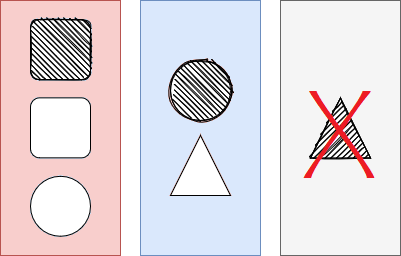
\includegraphics[width=0.6\textwidth]{images/empacotador_novo.png}
    \legend{Fonte: Autor.}
    \label{fig:method}
\end{figure}
\label{example::robo}
\end{example}

\begin{example}
Agora vamos estender o exemplo \ref{example::robo} supondo que o sensor tátil não está funcionando corretamente, e ele irá sentir objetos lisos como se fossem ondulados. Para nosso exemplo, vamos considerar que o primeiro item será um triângulo liso. Nenhum erro ocorre quando a câmera percebe o triângulo, mas o sensor tátil indica que ele é ondulado. Nesse caso, teremos uma ilusão, pois triângulo é um objeto válido, mas ele foi percebido com uma propriedade inválida, que não existe no contexto do agente. Não há planos para quando o agente detecta esse tipo de erro, então ele pode executar um plano padrão para casos de erro, ou simplesmente não fazer nada.
\label{example::ilusao1}
\end{example}{}

Esse tipo de anomalia demonstrado no Exemplo \ref{example::ilusao1} será chamado de ilusão classe 1, onde o corpo do predicado, ou o objeto da percepção, é válido, mas possui um argumento ou uma característica inválida.

\begin{definition}{}
   Uma ilusão classe 1 é uma percepção do tipo \texttt{objeto(caracteristica)} ou equivalente, onde \texttt{objeto} é um elemento do contexto do agente e \texttt{característica} não é.
\end{definition}

\begin{example}
    Se considerarmos que as percepções do agente possuem formas erradas por conta de um defeito na câmera ou o software de reconhecimento de padrões que atua sobre ela, um objeto como um círculo liso pode ser reconhecido como um estrela listrada. Estrela não é um objeto válido, mas listrado é.
    \label{example::ilusao2}
\end{example}{}

Isso será chamado de ilusão classe 2, definido de maneira similar a ilusão classe 1.

\begin{definition}{}
   Uma ilusão classe 2 é uma percepção do tipo \texttt{objeto(caracteristica)} ou equivalente, onde \texttt{objeto} não é um elemento do contexto do agente e \texttt{característica} é.
\end{definition}

Portanto, podemos simplesmente definir ilusão da seguinte forma:

\begin{definition}{}
   Uma ilusão é uma percepção do tipo \texttt{objeto(caracteristica)} ou equivalente, que se caracteriza como uma ilusão classe 1 ou uma ilusão classe 2.
\end{definition}

\subsubsection{Alucinação}

O segundo tipo de anomalia é a alucinação. Uma alucinação é uma percepção recebida que poderia ser completamente válida, mas que na realidade não existe no ambiente.

\begin{example} {}
    Retornando ao exemplo \ref{example::ilusao1} do agente responsável por empacotar os itens, mas que agora apresenta também o comportamento defeituoso do exemplo \ref{example::ilusao2}. Uma percepção formalmente correta, do tipo \texttt{objeto(caracteristica)}, por conta dos erros que os sensores possuem, pode resultar na percepção \texttt{estrela(ondulada)}. Essa percepção poderia ser processada pelo agente, entretanto ela não faz parte de seu contexto e resultaria na execução de um plano padrão para erros ou na inação do agente.
    \label{exemple::alucinacao}
\end{example}

Assim, vamos definir alucinação como um tipo específico de ilusão classe 1 e classe 2, podendo acarretar os mais diversos tipos de erros dentro do raciocínio do agente, ou gerando problemas caso seja ignorada.

\begin{definition}{}
   Uma alucinação é uma percepção do tipo \texttt{objeto(caracteristica)} ou equivalente, onde nem \texttt{objeto} nem \texttt{característica} são elementos do contexto do agente.
\end{definition}

\section{Planejamento automatizado}

Planejamento automatizado é um dos problemas fundamentais da Inteligência Artificial. As motivações para usar o planejamento automatizado são a capacidade de utilizar recursos de planejamento acessíveis e eficientes e reproduzir uma parte do processo cognitivo humano com um componente totalmente integrado de comportamento deliberativo \cite{GHALLAB20041}. A maneira clássica de realizar planejamento automatizado é considerar esse um problema de dedução lógica, onde dado um estado inicial, ações que aferam esse estado e um conjunto de estados de objetivo, é necessário encontrar a sequência de ações que faziam com que o ambiente saísse de um estado inicial para um estado de objetivo \cite{MADANI20035}.

Uma forma alternativa de tratar o problema de planejamento automatizado é utilizando planejamento probabilístico \cite{KUSHMERICK1995239}. Essa abordagem pode ser necessária por conta do fato de que o agente provavelmente não tem conhecimento completo do mundo ao seu redor. Outra saída para o problema do planejamento automatizado são os processos de decisão de Markov \cite{Cassandra:1998:EAA:926710}, \cite{DBLP:journals/corr/abs-1105-5460}, \cite{article}.

Na Definição \ref{definition::autoplanning} é apresentada a noção abstrata de planejamento automático, descrita como um modelo conceitual simples que contém os elementos principais do problema, tendo sido originalmente apresentada por Ghallab et. al. \cite{GHALLAB20041}.

\begin{definition}{}
\label{definition::autoplanning}
   % USAR MAIS TARDE PARA DEFINIR O BLOCO DE AUTOPLANEJAMENTO An automated planning block is a instance of the conceptual model of automated planning, described through the interaction between three components bellow \cite{GHALLAB20041}:
   Um modelo conceitual de planejamento automatizado é descrito como a interação entre os seguintes três componentes:
   
    \begin{itemize}
        \item Um sistema de transição de estados $\Sigma$, especificado por uma função de transição de estados $\Gamma$, de acordo com os eventos e ações que ele recebe. 
        \item Um $controlador$, que dado uma entrada de estados $s$ do sistema, fornece como saída uma ação de acordo com algum plano.
        \item Um $planejador$, que dado uma entrada de uma descrição de sistema $Z$, uma situação inicial e alguns objetivos, sintetiza um plano para o controlador a fim de alcançar o objetivo.
    \end{itemize}
    
    Um sistema de transição de estados $\Sigma$ é uma quádrupla $\Sigma = \langle S, A, E, \Gamma \rangle$, onde:
    
    \begin{itemize}
        \item $S = \{s_1, s_2, ..., s_{n}\}$ é um conjunto finito ou recursivamente enumerável de estados;
        \item $A = \{a_1, a_2, ..., a_{n}\}$ é um conjunto finito ou recursivamente enumerável de ações;
        \item $E = \{e_1, e_2, ..., e_{n}\}$ é um conjunto finito ou recursivamente enumerável de eventos; e 
        \item $\Gamma: S \times A \times E \rightarrow 2^S$ é uma função de transição de estados. 
    \end{itemize}
     
\end{definition}

\section{Resumo}

Existem diversas definições de agente, mas para este trabalho será considerado que um agente inteligente é uma entidade, inserida em um ambiente, que possui autonomia para tomar suas decisões. Essa entidade possui um conjunto de conhecimentos a respeito do ambiente, e pode atualizar esses conhecimentos através da percepção, o processo de utilizar seus sensores para reconhecer o mundo ao seu redor. O funcionamento básico de um agente acontece através da entrada de percepções novas, o processamento delas para atualizar a base de conhecimentos e a escolher de quais ações tomar. Como o agente pode receber muitas percepções de uma vez, pode ser necessário criar medidas para reduzir esse volume de acordo com certos parâmetros -- chamamos isso de refinamento.

Por fim, as percepções que um agente recebe podem ser anomalias, i. e., inválidas ou corrompidas. Separamos essas anomalias entre ilusões e alucinações, de acordo com suas características semânticas. Neste trabalho, será proposto um modelo que recebe as percepções, refina, detecta e classifica possíveis anomalias e cria novos planos para lidar com essas percepções inválidas através de um processo de planejamento automatizado.

Esse processo de receber percepções, categorizá-las como percepções válidas ou anomalias e gerar novos artefatos de valor para o agente é o que chamamos neste trabalho de revisão de percepções. No Capítulo \ref{chapter:relacionados} alguns trabalhos que propõem processos similares a revisão de percepções serão apresentados.